% Chapter 2
\chapter{State of the Art}
\label{chap:Chapter2}

This chapter is divided into three parts. 
Part I starts on the theoretical side by introducing Machine Learning, Security Operation Centers, Security Information and Event Managers, and response mechanisms such as \gls{IPS}, \gls{IDS}, and \gls{EDR}. 
It also explains how popular \gls{ML} classification models work and how to evaluate them. 
Understanding these topics is the groundwork for material considered later in the chapter.

The second part focuses on the automatic classification of security alert tickets. 
It begins with an overview of proposed solutions and then reviews several publicly available studies. 
The chapter concludes with a detailed evaluation of existing systems that are similar to the one presented in this thesis. 

The third and final part discusses existing technologies that \gls{SOC} may utilize. 
These technologies are designed to support the workflow outlined in the first section about \gls{SOC}. 
At least three different technologies will be presented and discussed for each aspect of the \gls{SOC} workflow. 
The section will conclude with a summary of the key differences among the technologies and, if relevant, evaluate which one may be superior.

\section{Theoretical Introduction}

Before diving into the technologies, tools, and methodologies used for automating the classification of security alert tickets, it is essential to understand some fundamental concepts. 
Concepts like, \gls{SOC}s, \gls{SIEM} systems, \gls{AI}, particularly \gls{ML}, and advanced threat detection and response mechanisms. 
Such a foundation is indispensable for comprehending these systems' functions, construction work, advantages and limitations, and the actual performance comparison among different methods. 
The chapter introduces \gls{SOC} and how it functions, then moves on to the foundations of \gls{ML} and provides an overview of models frequently used for classification problems. 
It provides an overview of methods for assessing the performance of classification models, placing this in context for their use within the project.

\subsection{Security Operations Center} 

The complexity and frequency of cyber threats are increasing \parencite{Arianna2024}, which has led to the emergence of \gls{SOC}s as a critical component of modern IT enterprises. 
\gls{SOC}s are the primary defenders in incident response planning, vulnerability management, and regulatory compliance. 
In today's interconnected world, integrating security operations to reduce defensive barriers allows organizations to optimize resources, enhance security posture, and safeguard critical assets.

A \gls{SOC} is a unit \parencite{Rutledge2024} that provides tailored and centralized \gls{CND} \parencite{Zimmerman2014}. 
It defends computer networks against the growing world of cyber threats. 
The main objective of a \gls{SOC} is to ensure continuous monitoring and incident response for enterprise systems \parencite{Zimmerman2014}. 
This primarily focuses on preventing unauthorized access, cyber-attacks, and data breaches.

This \gls{24/7} facility leverages advanced technologies and skilled information security professionals to monitor the network continuously \parencite{Zimmerman2014}. 
With sophisticated tools to detect anomalies, a \gls{SOC} can address threats before they escalate.

\subsubsection{Definition and Characteristics of a SOC}
\textcite{Zimmerman2014} defined a \gls{SOC} as:
\begin{quote}
    ``A team primarily composed of security analysts organized to detect, analyze, respond to, report on, and prevent cybersecurity incidents.''
\end{quote}

This definition integrates elements from various sources, including the historical definition of \gls{CSIRT} as detailed in references \parencite{Shirey2007} and \parencite{Brownlee1998}. 

For an organization to qualify as a \gls{SOC}, according to \textcite{Zimmerman2014}, it must:
\begin{enumerate}
    \item Establish a system for constituents to report cybersecurity incidents.
    \item Provide comprehensive support for managing and resolving incidents effectively.
    \item Convey incident-related information to internal and external stakeholders.
\end{enumerate}

\subsubsection{Key Responsibilities of a SOC}
A \gls{SOC} has several critical missions, as outlined by various sources \parencite{Muniz2015, Zimmerman2014}:
\begin{itemize}
    \item Preventing cybersecurity incidents by implementing proactive measures such as vulnerability scanning and threat analysis.
    \item Monitor, detect, and analyze potential security intrusions.
    \item Handle confirmed incidents and coordinate resources for effective countermeasures.
    \item Providing stakeholders with situational awareness regarding cybersecurity incidents, trends, and threats.
\end{itemize}

\subsubsection{Tiers of Operation}
Analysts within a \gls{SOC} operate in tiers \parencite{Vielberth2020}. 
Tier 1 analysts monitor and conduct initial investigations, escalating complex cases to Tier 2 analysts, who perform in-depth analyses and take further actions like blocking activities or deactivating accounts. 
Generally, higher-tier analysts handle more complex incidents, which require more time to resolve.

\begin{figure}[ht]
    \centering
    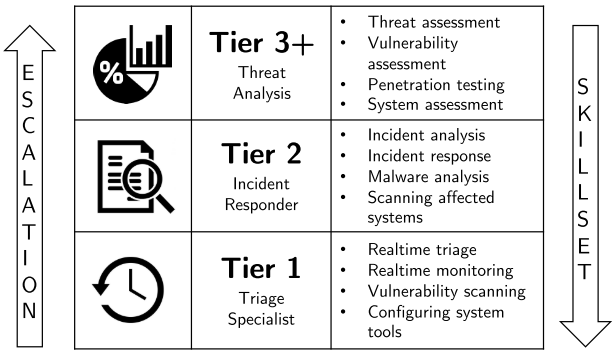
\includegraphics[width=\textwidth]{ch2/assets/tierTable.png}
    \caption{SOC Analyst Tier Responsibilities, from \autocite{Kokulu2019}.}
    \label{fig:soc-tier}
\end{figure}

Extra levels may exist that handle responsibilities like threat hunting, vulnerability assessments, and penetration testing. 
These levels are collectively termed Tier 3+. 
Figure~\ref{fig:soc-tier} was taken from a paper on a qualitative study on a \gls{SOC} \parencite{Kokulu2019} and illustrates a visual representation of these tiers and their associated tasks. 
Not all \gls{SOC}s follow a hierarchical model. 
In some collaborative frameworks, team members may possess comparable skill sets, enabling them to manage incidents independently \parencite{Kokulu2019}.

\subsubsection{Triage Specialist}

Since this project focuses on automating the triage process, it is crucial to gain a detailed understanding of the role of a triage specialist, their functions, and the advantages of automated triage in comparison.

Tier 1 analysts, also known as triage specialists, play a critical role in the initial stages of a \gls{SOC} workflow \parencite{Vielberth2020}. 

As stated by \textcite{Vielberth2020}, a Tier 1 analyst's primary responsibilities include:
\begin{enumerate}
    \item Collecting and analyzing raw data.
    \item Reviewing alarms and alerts generated by monitoring systems.
    \item Determining the validity and criticality of each alert.
\end{enumerate}

They must improve alerts with additional contextual information and decide whether an alert represents a real threat or a false positive \parencite{Hamornik2018, Sundaramurthy2014}. This process demands meticulous attention to detail, as the triage specialist must assess individual alerts, notify potential high-risk events, and prioritize them according to their severity \parencite{Tao2018}. 

The repetitive nature of triage work, coupled with the need to escalate unresolved issues to Tier 2 analysts, can result in mental fatigue and burnout \parencite{Tines2023, Iamnitchi2017}. This exhaustion affects individual performance and can compromise the overall efficiency of the \gls{SOC}, as delayed or missed alerts may result in critical threats going undetected \parencite{CriticalStart2019}.

In a 2018 study \parencite{Crowley2018}, 53\% of respondents in a security survey identified inadequate automation as the most common shortcoming.

This study demonstrates that effectively structured and implemented automation can help mitigate some or many of a \gls{SOC}'s weaknesses, particularly in the repetitive aspects of the \gls{SOC}'s workflow, such as the triage process.

\subsection{Security Information and Event Management}

The increasing complexity of cybersecurity threats has compelled organizations to implement advanced technologies to protect their digital assets. 
\gls{SIEM} systems have emerged as vital tools in this context \parencite{Shaw2022}.

\gls{SIEM} systems gather and centralize security-related data to detect threats and respond to incidents effectively. 
These systems connect logs from various sources to support security analytics, enabling real-time monitoring and retrospective analysis of past events \parencite{Shaw2022}.
They integrate with cyber threat intelligence platforms, providing human analysts with advanced visual tools for seamless information sharing between organizations. 
Additionally, they retain event data over extended periods, ensuring robust log management capabilities.

The key features of a \gls{SIEM} system, as gathered from various published sources \parencite{Harper2010, Sheeraz2023, Ali2024}, are:

\begin{itemize}
    \item \textbf{Log Collection:} SIEM gathers log data from various network devices such as servers, firewalls, and switches. Data can be collected using two methods:
    \begin{enumerate}
        \item \textbf{Agent-based collection:} An intermediary agent collects and forwards logs.
        \item \textbf{Agent-less collection:} Servers retrieve logs directly from the source devices.
    \end{enumerate}
    
    \item \textbf{Log Aggregation:} Collected logs are analyzed and structured for meaningful insights. Aggregation methods include:
    \begin{enumerate}
        \item \textbf{Push method:} Devices actively send logs to the SIEM.
        \item \textbf{Pull method:} SIEM retrieves logs as needed.
    \end{enumerate}
    
    \item \textbf{Parsing and Normalization:} Parsing converts raw logs into structured data, while normalization standardizes logs from diverse sources to eliminate redundancy.
    
    \item \textbf{Threat Analysis and Detection:} By correlating log data with known threat indicators, SIEM systems identify malicious activities. Statistical methods and predefined rules enhance their ability to detect sophisticated threats.
    
    \item \textbf{Response Automation:} SIEM systems issue real-time alerts and notifications, enabling rapid responses to potential incidents.
    
    \item \textbf{Reporting and Visualization:} Advanced reporting tools provide security analysts with actionable insights, enabling detailed investigations and trend analysis.
\end{itemize}

\subsubsection{Architectural Components}

The architectural components of a security information and Event Management (SIEM) system consist of several essential elements that enable effective security monitoring, incident detection, and response \parencite{Sheeraz2023}.

Data sources provide the raw material for analysis and threat detection \parencite{Ali2024}. These include a wide variety of log-generating devices and applications:
\begin{itemize}
    \item \textbf{Network devices}: Firewalls, routers, and switches.
    \item \textbf{Endpoint devices}: Workstations, servers, and mobile devices.
    \item \textbf{Applications}: Web servers, databases, and cloud platforms.
\end{itemize}

A variety of data sources is crucial for effective monitoring and threat detection. 

\textbf{Data collection} is a vital step with two main approaches to consider:
\begin{itemize}
    \item \textbf{Agent-based collection}: Agent-based collection uses proxy agents on endpoint devices for better control and flexibility in log collection, but it is costly and complex to manage.
    \item \textbf{Agent-less collection}: Agent-less collection allows devices to send data directly to the SIEM, simplifying deployment but may reduce efficiency in high-volume data environments.
\end{itemize}

The \textbf{SIEM processing engine} is one of the critical components \parencite{Sheeraz2023} responsible for:
\begin{itemize}
    \item \textbf{Parsing}: The conversion of raw log data into a structured format used for analysis.
    \item \textbf{Normalization}: Ensure the log formats are standardized to facilitate easier comparisons.
    \item \textbf{Correlation}: Finding relationships between events to strengthen security posture or incident response.
\end{itemize}

\textbf{Storage and rationalization} are vital for ensuring scalability and compliance. SIEM systems must store logs for future analysis.
This means there has to be enough storage and a logical way of organizing this data for scalability or compliance requirements like GDPR and HIPAA \parencite{Sheeraz2023}.
Effective storage solutions should scale dynamically to handle large datasets without compromising performance or compliance standards.

\textbf{Visualization and reporting tools} play a key role in making data accessible and actionable.
Critical functions that significantly benefit from good data visualization and reporting tools are incident investigation, trend analysis, and compliance audits \parencite{Sheeraz2023}. 
These features not only improve user experience but also aid in making data actionable and accessible. 
Organizations can use these tools to conduct incident investigations, identify patterns occurring over time, and monitor compliance \parencite{Sheeraz2023}. 
This comprehensive approach enables the development of scalable systems that can effectively handle increasing data demands.

\clearpage

\begin{figure}[ht]
    \centering
    
\includegraphics[width=\textwidth]{ch2/assets/FinalGraph.png}
    \caption{SIEM Architecture}
    \label{fig:siem-arc}
\end{figure}

Figure~\ref{fig:siem-arc} illustrates the architecture of a \gls{SIEM} system, highlighting its critical components and their interactions. 
Data flows from network and endpoint devices, as well as applications, to the log collection module. 
The \gls{SIEM} processing engine then parses, normalizes, and correlates this data for real-time security alert analysis, event monitoring, and threat detection.

The diagram also emphasizes the importance of visualization and reporting tools for turning data into actionable insights.

The graphic illustrates how these elements integrate into a SIEM.

\subsection{Machine Learning}

\gls{ML} is a core part of \gls{AI} but also overlaps with data mining, statistics, probability, and mathematics \parencite{Mohri2012}. 
Unlike traditional rule-based systems that rely on predefined logic, \gls{ML} uses induction—it learns patterns from past data and forms assumptions that can be generalized to new cases \parencite{Ali2024}. 
This method relies on datasets, which are groups of examples the \gls{ML} algorithm analyzes to find patterns \parencite{Mohri2012, Suthaharan2016}. 
The goal is to use these learned patterns to predict or describe new data.

There are three primary types of techniques employed in machine learning, \parencite{Mohri2012}:

\begin{enumerate}
    \item \textbf{Reinforcement Learning}: 
    This is a subset of machine learning in which an agent learns by interacting with the environment \parencite{Moradi2023}. It observes the environment, selects an action, and receives a reward if the action is beneficial or a penalty if it is detrimental. Over time, it refines its approach to achieve maximum rewards.

    \item \textbf{Supervised Learning}: 
    In this type of machine learning, models are trained on labeled data, meaning that each example includes input features and the corresponding expected output (or label). The model learns to map the inputs to the outputs, enabling it to predict the output for new, unseen data.

    \item \textbf{Unsupervised Learning}: 
    Unsupervised learning analyzes unlabeled data to reveal patterns without predefined labels. Unlike supervised learning, it allows algorithms to explore data independently. It is often used for clustering similar data points or modeling probability distributions. This approach is valuable for understanding the inherent organization in data without prior knowledge.
\end{enumerate}

Supervised learning can be further categorized into several types, \parencite{Mohri2012}:

\begin{itemize}
    \item \textbf{Regression}: 
    Regression algorithms predict numerical values within a continuous range by analyzing input data to identify patterns. They can forecast future values, such as calculating the next number in a sequence based on previous numbers and trends. Techniques like linear regression, polynomial regression, and others enable these algorithms to draw conclusions and make predictions effectively.
    
    \item \textbf{Similarity}: 
    Similarity algorithms analyze and compare two distinct instances to measure their resemblance. They are vital in recommender systems for suggesting products based on user preferences and in visual identity tracking and verification by comparing images or features. Their versatility makes them essential in data analysis, security, and personalized user experiences.
    
    \item \textbf{Classification}: 
    Classification algorithms classify the input data into predefined groups. Classification tasks can be binary when there are only two possible categories (such as a yes-no decision) or multiclass when the number of categories exceeds two, such as recognizing handwritten letters in the alphabet.
\end{itemize}

However, \gls{ML} has its limitations. 
Since datasets are finite, no algorithm can predict every scenario, which highlights an essential aspect of inductive reasoning: it can suggest likely outcomes but cannot ensure certainty \parencite{Mohri2012, Suthaharan2016}. 

In \gls{ML}, achieving an optimal model involves balancing between two critical concepts: \textbf{bias} and \textbf{variance}. 
Bias refers to the error introduced when a model is excessively simplistic, which can lead to underfitting. 
Underfitting occurs when the model fails to capture the underlying patterns of the data, resulting in poor performance on both training and unseen datasets \parencite{ElSahly2023}. 
On the other hand, variance arises when a model becomes overly complex and sensitive to the fluctuations in the training data, culminating in overfitting. 
Overfitting means the model performs exceptionally well on the training dataset but poorly on new, unseen data because it has memorized the noise instead of learning the actual signal \parencite{ElSahly2023}. 

The primary objective in constructing a machine learning model is to identify the appropriate level of complexity with the right balance, ensuring the model generalizes well and performs effectively on new data \parencite{Suthaharan2016}.

Despite these challenges, \gls{ML} continues to evolve, with increasingly sophisticated algorithms enabling breakthroughs in many fields \parencite{Mohri2012}. 

\subsection{Machine Learning Models}

The processes and computations of training a machine learning model are structured within a framework. 
This chapter will briefly overview the most frequently used algorithms relevant to this project's goals.

\subsubsection{Decision Trees}

Decision Trees (DTs) are a fundamental supervised machine learning algorithm for classification and regression tasks \parencite{Huang2024}. 
They work by splitting data into subsets based on the value of input features, forming a tree-like structure composed of nodes and branches.

The process begins at the root node, representing the entire dataset, and iteratively divides the data into homogeneous subsets using decision nodes until a terminal leaf node is reached, representing the output prediction or class \parencite{Chauhan2022}, as seen in Figure~\ref{fig:struc-DT}.

\begin{figure}[h]
    \centering
    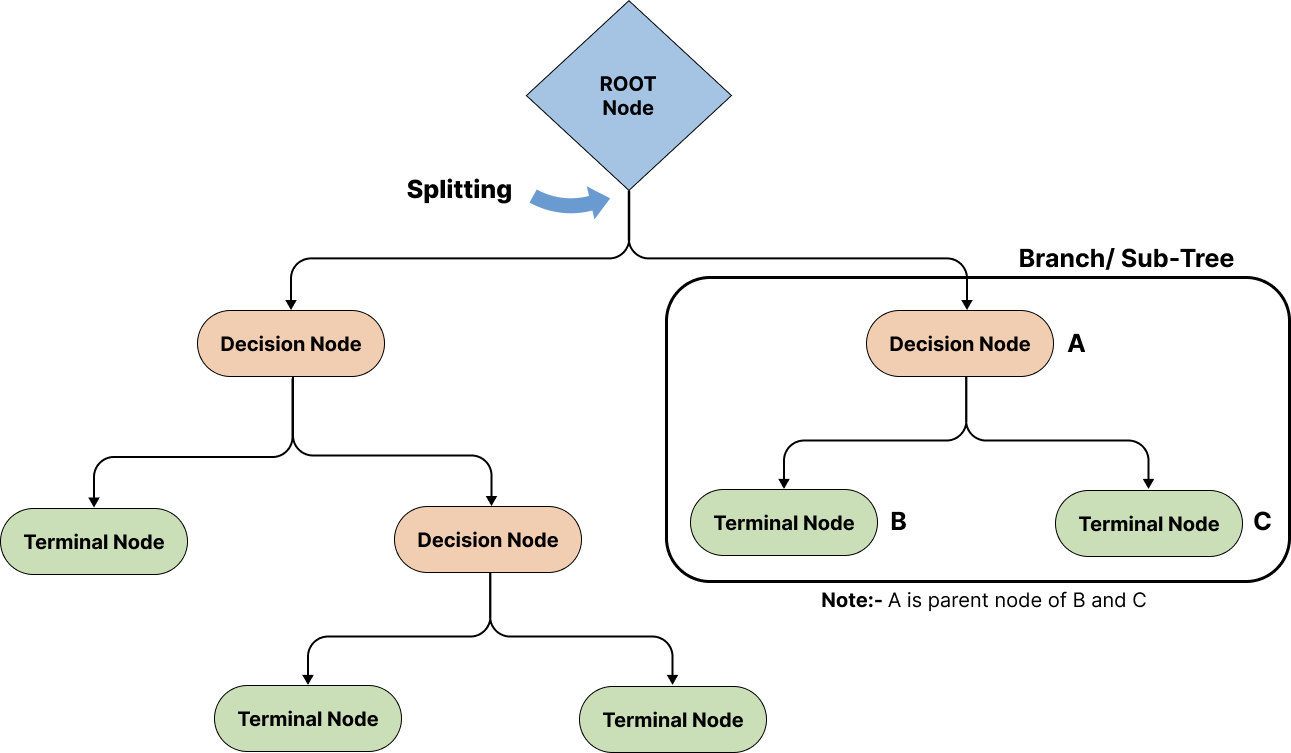
\includegraphics[width=\textwidth]{ch2/assets/FinalTreeGraph.png}
    \caption{A basic structure of a Decision Tree, based on \parencite{Chauhan2022}}
    \label{fig:struc-DT}
\end{figure}

The algorithm operates by evaluating all potential splits and selecting the one that optimizes a specific criterion, such as information gain or Gini impurity. 
Information gain measures the reduction in entropy after a split, while Gini impurity quantifies the likelihood of misclassification at a node. 

The entropy of \( S \) is defined as:
\begin{equation}
H(S) = \sum_{i=1}^{n} -P(s_i) \times \log_b P(s_i)
\end{equation}
where \( S \) is a set of values \( s_1, s_2, \dots, s_n \), \( P(s_i) \) is the probability of observing a certain value, and \( b \) is the logarithm base, most commonly \( 2 \), \( e \), or \( 10 \).

Using entropy, the \textbf{information gain (IG)} for a node \( t \) and a candidate split \( x \) is calculated as:
\begin{equation}
IG(t, x) = H(t) - H(x, t)
\end{equation}
In contrast, the \textbf{Gini index}, another commonly used metric for evaluating splits, is defined as:
\begin{equation}
\text{Gini} = 1 - \sum_{i=1}^{n} P(s_i).
\end{equation}

At each decision node, the algorithm tests a single feature and branches according to its value, guiding data instances down the tree until they reach a leaf node \parencite{Chauhan2022}. 
During training, the algorithm continues splitting until a stopping criterion is met, such as achieving a maximum tree depth, minimum node size, or no further improvement in the splitting metric \parencite{Chauhan2022}.

Pruning techniques prevent overfitting, which occurs when a tree becomes too complex and overly specific to the training data. 
These involve removing unnecessary branches or nodes to simplify the tree while maintaining predictive accuracy. 
Pruning can be preemptive (stopping tree growth early) or post hoc (removing branches after the tree is fully grown). 
This ensures that the decision tree generalizes well to unseen data \parencite{Huang2024}.

Decision trees are non-parametric, meaning they do not assume any specific distribution for the data, and they can capture both linear and non-linear relationships \parencite{Huang2024}. 
However, they are sensitive to slight variations in the dataset \parencite{Huang2024}, which may cause significant changes in the tree structure. 
Despite this, they remain popular for their simplicity, interpretability, and ability to handle numerical and categorical data \parencite{Chauhan2022}.

\subsubsection{Ensemble classifiers}

Ensemble learning is a powerful machine learning technique that combines the predictions of multiple base models to achieve superior performance compared to individual learners \parencite{Joseph2022}.

The fundamental idea is to address the limitations of single models, such as high variance, high bias, or low accuracy, by leveraging the diversity and complementary strengths of multiple models \parencite{Mienye2022, Dasarathy1979, Hansen1990}.

The concept of ensemble learning has evolved significantly since its inception. Early work by \textcite{Dasarathy1979} introduced the partitioning of feature spaces using multiple classifiers. 
Later, \textcite{Hansen1990} demonstrated that ensembles of artificial neural networks achieved superior predictive performance compared to single networks. 
\textcite{Schapire1990} groundbreaking work laid the foundation for boosting, one of the primary techniques in ensemble learning.

Ensemble learning methods are evaluated on two main principles: \textbf{accuracy} and \textbf{diversity} of the base learners \parencite{Hansen1990, Mienye2022}.

\begin{itemize}
    \item \textbf{Accuracy}: Each base learner should perform better than random guessing on the given task \parencite{Li2012}.
    \item \textbf{Diversity}: The errors made by individual learners should be uncorrelated, which can be achieved through techniques like subsampling, feature randomization, or algorithmic diversity \parencite{Schapire1990, Breiman1996}.
\end{itemize}

A model is accurate if it generalizes well on unseen instances, while diversity ensures that the errors of individual base models are not correlated. 
Achieving this balance is crucial for effective ensembles.

Ensemble Classifiers offer several advantages over single models, making them a popular choice in diverse applications of machine learning:
\begin{itemize}
    \item \textbf{Improved Generalization}: Ensembles reduce overfitting and improve generalization by aggregating the predictions of multiple learners \parencite{Hansen1990}.
    \item \textbf{Bias-Variance Trade-off}: Techniques like bagging reduce variance while boosting minimizes bias, addressing the critical limitations of individual learners \parencite{Li2012, Mienye2022}.
    \item \textbf{Adaptability}: Ensembles can be designed to work with homogeneous (same algorithm) or heterogeneous (different algorithms) base learners, making them versatile across domains \parencite{Mienye2022}.
\end{itemize}

Ensemble learning methods are broadly categorized into:
\begin{itemize}
    \item \textbf{Parallel Ensembles}: Base learners are trained independently on different subsets of data or features. Techniques like bagging and Random Forests fall into this category \parencite{Breiman1996}. The illustration in Figure~\ref{fig:parallel_emsemble} demonstrates how parallel ensembles operate.
    \item \textbf{Sequential Ensembles}: Models are trained iteratively, with each learner focusing on correcting the errors of its predecessor. Boosting is the most prominent example of this approach \parencite{Schapire1990}. The illustration in Figure~\ref{fig:sequential_emsemble} demonstrates how sequential ensembles operate.
    \item \textbf{Stacked Ensembles}: Predictions from multiple base models are combined using a meta-model trained on the outputs of the base learners \parencite{Mienye2022}.
\end{itemize}

\begin{figure}[b!]
    \centering
    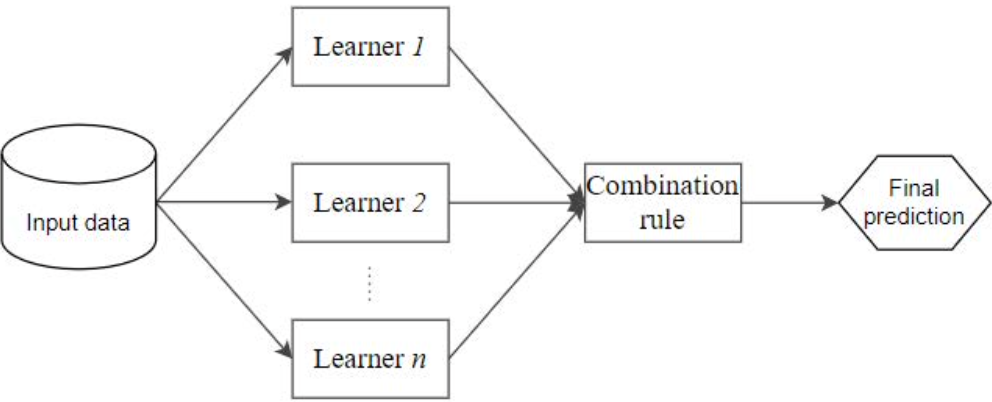
\includegraphics[width=\textwidth]{ch2/assets/Block_diagram_of_parallel_ensemble_learning.png}
    \caption{Diagram of Parallel Ensemble Learning from \parencite{Mienye2022}}
    \label{fig:parallel_emsemble}
\end{figure}

\clearpage

\begin{figure}[t!]
    \centering
    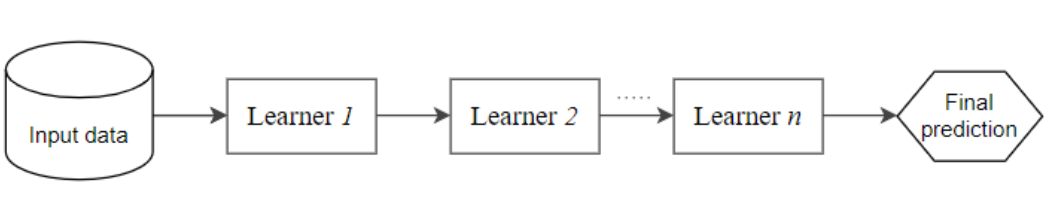
\includegraphics[width=\textwidth]{ch2/assets/Block_diagram_of_sequential_ensemble_learning.png}
    \caption{Diagram of Sequential Ensemble Learning. from \parencite{Mienye2022}}
    \label{fig:sequential_emsemble}
\end{figure}

Ensemble methods can then be categorized into three main approaches based on how they train and combine base models: \textbf{Bagging}, \textbf{Boosting}, and \textbf{Stacking}. 
Each method has a distinct mechanism for generating diversity and aggregating predictions, addressing the specific limitations of single models.

\paragraph{Bagging}
Bagging, which stands for bootstrap aggregating, is a parallel ensemble technique where multiple base models are independently trained on random subsets of the training data, referred to as bootstrapped samples. 
The final predictions are made by aggregating the outputs of these models, often using majority voting or averaging. 
Random Forests are a well-known implementation of bagging, recognized for their ability to reduce variance without increasing bias \parencite{Mienye2022}.

\paragraph{Boosting}
Boosting is a sequential ensemble method that aims to reduce bias by iteratively training base models. 
Each subsequent model focuses on correcting the errors made by the previous one, assigning higher weights to misclassified samples. 
Algorithms such as AdaBoost and Gradient Boosting exemplify this approach, often achieving superior performance on complex datasets, but this can lead to increased susceptibility to overfitting \parencite{Mienye2022}.

\paragraph{Stacking}
Stacking integrates predictions from multiple base models using a meta-model that learns the optimal way to combine their outputs. 
Unlike bagging and boosting, stacking allows for heterogeneous base learners, providing greater flexibility and diversity. 
The meta-model is typically trained on the predictions made by the base models, enabling it to make more accurate decisions \parencite{Mienye2022}.

\subsubsection{Random Forests}

Random Forests represent a significant advancement in machine learning, particularly in the domain of ensemble classifiers \parencite{Ali2024}. 

As a bagging-based ensemble method, Random Forests combine multiple decision trees to improve classification accuracy and robustness. 
This approach leverages the strengths of individual trees while mitigating their limitations, such as overfitting, by aggregating their predictions \parencite{Ali2024}. 

The Random Forest algorithm begins by generating multiple decision trees, as can be seen on Figure~\ref{fig:random_forest_algorithm}, each trained on a random subset of the training data through bootstrapping\footnote{Bootstrapping is a resampling technique where random samples are drawn with replacement from the dataset.}.
Additionally, features are randomly sampled at each split to ensure diversity among the trees, a process that reduces the correlation between individual tree predictions \parencite{Farooq2018}. 
Once trained, the predictions of all trees are aggregated, typically through majority voting for classification tasks or averaging for regression tasks, to produce the final output \parencite{Nila2020}. 

\begin{figure}[h!]
    \centering
    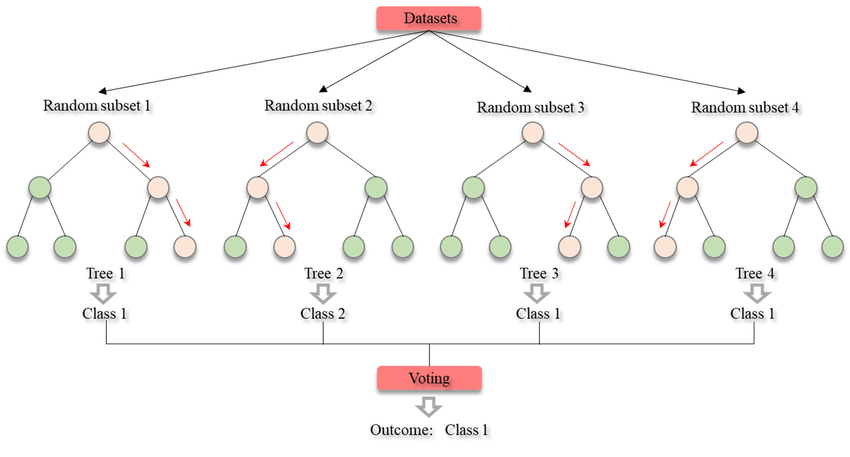
\includegraphics[width=\textwidth]{ch2/assets/Workflow-of-the-random-forest-algorithm.ppm.png}
    \caption{Workflow of Random Forests: Bootstrapping, Decision Trees, and Aggregated Predictions from \parencite{Yang2019}}
    \label{fig:random_forest_algorithm}
\end{figure}

Random Forests are highly valued for their versatility and robustness. 
They perform exceptionally well with large and high-dimensional datasets, effectively handling numerical and categorical data. 
Furthermore, their inherent ability to measure feature importance makes them interpretable, a critical requirement in security domains where trust and explanation are essential \parencite{Ali2024}. 

Random Forests also excel at reducing overfitting, a common issue with individual decision trees. 
By averaging the predictions of multiple trees, the model achieves better generalization, even when faced with noisy data \parencite{Sopan2019}. 

Random Forests have been widely adopted in cybersecurity applications, particularly for detecting anomalies, classifying alerts, and predicting the likelihood of malicious behavior. 
For example, they are effectively used in \gls{SIEM} systems to process large volumes of log data, identify patterns, and reduce false positives \parencite{Farooq2018, Ali2024}. 

Studies have shown that Random Forest-based models can achieve high accuracy in detecting advanced persistent threats (APTs) and other cyberattacks by leveraging their ability to handle complex feature interactions and high-dimensional data \parencite{Ali2024}. 
For instance, combining Random Forests with additional modules for feature selection and preprocessing has improved detection rates and reduced manual intervention in incident response workflows \parencite{Nila2020}.

\subsubsection{Naive Bayes}

The Naive Bayes algorithm is a probabilistic classifier based on Bayes' theorem, which assumes conditional independence among features given the class \parencite{Chandra2016}.
This simplicity makes it computationally efficient and easy to implement. 

Naive Bayes is particularly effective in scenarios where the assumption of feature independence is approximately attained, such as spam detection and document classification. 
The model's reliance on this assumption allows it to scale effectively to high-dimensional datasets while remaining computationally efficient \parencite{Chandra2016}.

Naive Bayes calculates the posterior probability of each class given the observed data using the formula:

\begin{equation}
P(C|X) = \frac{P(X|C) \cdot P(C)}{P(X)}
\end{equation}

where:
\begin{itemize}
    \item \( P(C|X) \) is the posterior probability of class \( C \) given the feature vector \( X \),
    \item \( P(X|C) \) is the likelihood of observing \( X \) given class \( C \),
    \item \( P(C) \) is the prior probability of class \( C \),
    \item \( P(X) \) is the probability of the feature vector \( X \).
\end{itemize}

In practice, the Naive Bayes model, Figure~\ref{fig:naive_bayes}, estimates the prior probability \( P(C) \) for each class and the conditional probability \( P(X_i|C) \) for each feature \( X_i \) given the class. 
These probabilities are typically derived from the frequency of occurrences in the training data. 
For continuous features, it is common to assume a Gaussian distribution and compute the likelihood accordingly. 
The model assigns a new instance to the class with the highest posterior probability \( P(C|X) \) \parencite{Nila2020, Chandra2016}.

\begin{figure}[h!]
    \centering
    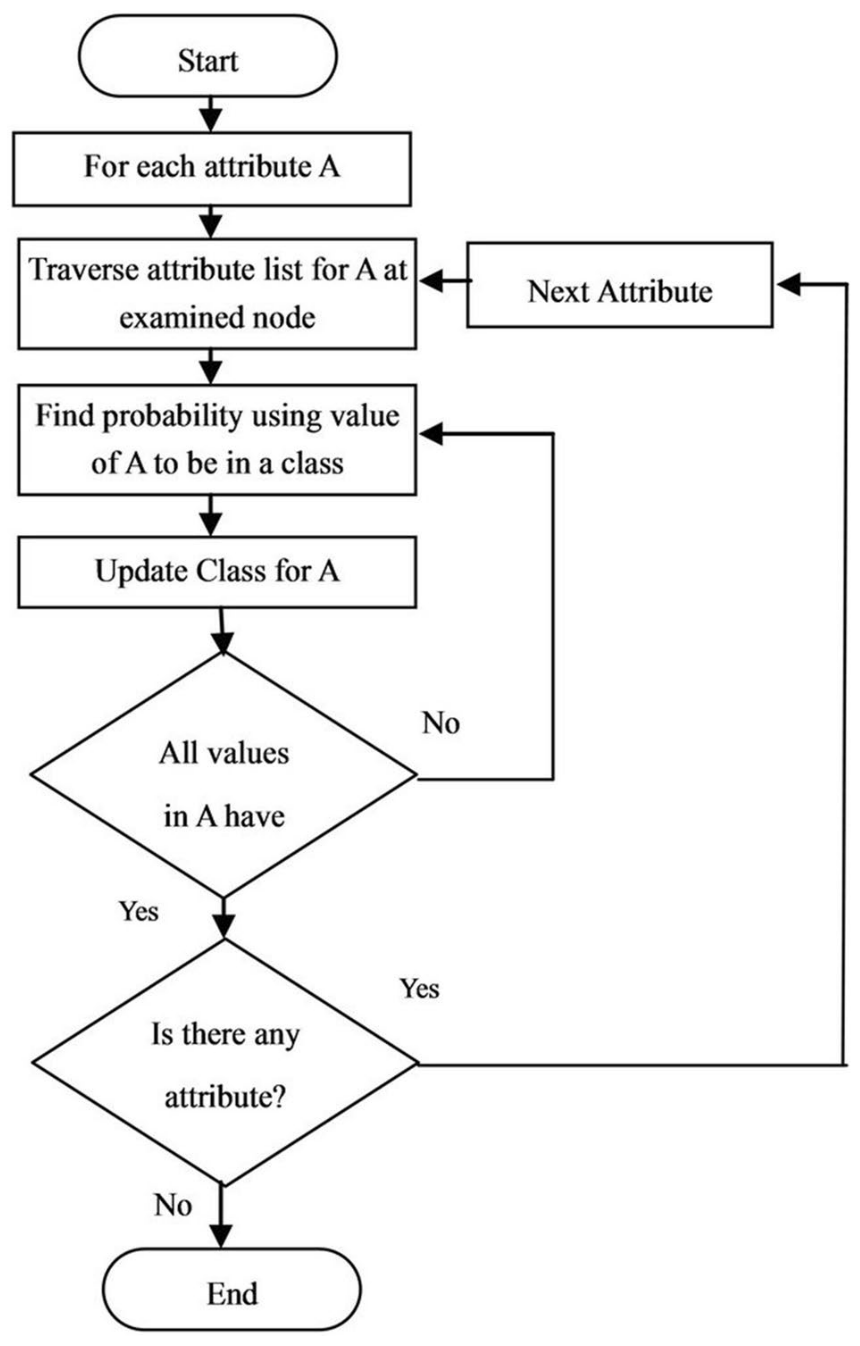
\includegraphics[width=0.3\textwidth]{ch2/assets/Flow-chart-for-Naive-Bayesian-classification.png}
    \caption{Schematic Diagram of the Naive Bayes Classification Process from \parencite{Sneha2019}}
    \label{fig:naive_bayes}
\end{figure}

This decision rule is computationally efficient, making Naive Bayes suitable for real-time prediction tasks \parencite{Nila2020, Chandra2016}. 

However, the strong independence assumption may only hold in some scenarios, potentially leading to suboptimal performance when features are highly correlated. 
Despite this limitation, Naive Bayes remains popular due to its simplicity and effectiveness in many practical applications \parencite{Chandra2016}.

\section{Automatic Classification of Security Alerts in SOC}

The growing complexity of cyber threats, especially \gls{APT}, has led to significant advancements in automated detection and mitigation mechanisms. 
Many of these mechanisms utilize \gls{ML} techniques. 
This section examines key works, focusing on their methodologies, limitations, and relevance to the problem of alert triage automation in \gls{SOC}.

Recent research has explored hybrid approaches to anomaly detection. 
\textcite{Saini2023} proposed a hybrid ensemble model combining Random Forest and XGBoost classifiers, achieving a 99.91\% accuracy on the CIC-IDS2017\footnote{Labeled dataset of network traffic, including normal behavior and various attacks, used to evaluate intrusion detection models.} dataset with a False Positive Rate (FPR) as low as 0.12\%. 
Despite its high performance, the model relies on static datasets, which limits its adaptability to evolving attack patterns. 
Similarly, \textcite{Ghafir2018} developed Machine Learning for Advanced Persistent Threats (MLAPT), a multi-phase system incorporating correlation frameworks for APT detection, achieving an accuracy of 84.8\%. 
While this approach improved early-stage prediction, its accuracy was limited compared to ensemble methods and lacked scalability for dynamic environments.

\textcite{Ali2024} extended APT datasets to include a diverse range of alerts. 
They integrated Random Forest and XGBoost models into a SIEM environment, demonstrating the ability to reduce FPR and achieve a near-perfect 99.6\% accuracy. 
However, the computational demands of such systems may hinder practical deployment in resource-constrained environments.
On the contrary, \textcite{Brogi2016} utilized Information Flow Tracking (IFT) for APT detection, concentrating on the correlation between the various stages of an attack. 
While this method excels at tracing complex multi-stage attacks, it requires further automation to support large-scale SOC operations effectively.

Incorporating reinforcement learning, \textcite{Sethi2020} introduced a Deep Q-Network (DQN)-based context-adaptive intrusion detection system, which improved FPR and demonstrated robustness against several attacks. 
Nevertheless, the distributed nature of their approach introduces practical deployment challenges, especially in SOC environments where centralized oversight is critical. 
Similarly, \textcite{Nila2020} explored ML-based triage systems to automate alert classification and reduce false positives. 
Their work effectively alleviated analyst fatigue by prioritizing actionable alerts, yet the scope of implementation remains limited to standalone systems.

\textcite{Chandra2016} conducted a comprehensive study on email-based APT entry points, explicitly exploring the effectiveness of Bayesian spam filters\footnote{Bayesian spam filters classify emails as spam or legitimate using probabilities based on Bayes theorem.}.
These filters demonstrated a strong capability to identify and differentiate between spear-phishing attempts and general spam emails, which is crucial for enhancing cybersecurity measures. 
However, the authors noted that while their solution provided significant benefits in detecting these specific types of email threats, it needed to address the broader range of APT life cycles.
This limitation restricts its effectiveness in SOC environments with diverse attack vectors, requiring a more holistic approach to threat detection and response strategies to encompass the full spectrum of APT strategies and tactics.

Table~\ref{tab:related_work_table} presents a detailed summary of the relevant studies explored, highlighting their respective strengths, weaknesses, and potential areas for enhancement.

\captionsetup[table]{font=small} % Set the caption font size
\scriptsize % Reduce the font size for the table content
\begin{longtable}{@{}P{1.9cm}P{1.9cm}P{1.9cm}P{1.9cm}P{1.9cm}P{3cm}@{}}
    \caption{Summary of the Existing Related Works based on \textcite{Ali2024}.}
    \label{tab:related_work_table} \\
    \toprule
    \textbf{References} & APT Life Cycle Coverage & AI Models Used & Lowest FPR & Highest Accuracy & Limitations \\
    \midrule
    \endfirsthead
    \toprule
    \textbf{References} & APT Life Cycle Coverage & AI Models Used & Lowest FPR & Highest Accuracy & Limitations \\
    \midrule
    \endhead
    \bottomrule
    \endfoot
    \bottomrule
    \endlastfoot
    \textcite{Ghafir2018} & Complete & Decision Tree, SVM, KNN, Ensemble Classifier & 4.5\% & 84.8\% & The blacklist-based detection modules require continuous update. Moreover, the accuracy is lower. \\
    \hline
    \textcite{Brogi2016} & Complete & No ML model used & High & Not calculated & Information Flow Tracking is used to detect APTs; however, the FPR is high. \\
    \hline
    \textcite{Giura2012} & Complete & No ML model used & 27.88\% & Not calculated & Sufficient knowledge is required to set up the mechanism. \\
    \hline
    \textcite{Sopan2019} & No & Random Forest & Not calculated & 98.5\% & The post-alert decision is not automated; it involves the intervention of security experts. \\
    \hline
    \textcite{Farooq2018} & Partial & SVM, Random Forest & Not calculated & Not calculated & The process anomaly detection is presented formally using One-Class SVM. However, the paper lacks ML-based experimental results. \\
    \hline
    \textcite{Sethi2020} & No & Deep Q-network & 0.35\% & 96.12\% & The proposed model enables the detection of APTs. \\
    \hline
    \textcite{Nila2020} & No & ZeroR, OneR, NaiveBayes, SVM, J48, RandomForest & Not calculated & 95.5\% & The authors did not discuss the FPR of the proposed model. \\
    \hline
    \textcite{Chandra2016} & Partial & NaiveBayes & Not calculated & 87\% & The authors did not discuss the FPR of the proposed model. \\
    \hline
    \textcite{Saini2023} & Partial & Random Forest, XGBoost & 0.12\% & 99.91\% & This study used existing datasets, posing a challenge because these datasets might not contain the latest attack scenarios. \\
    \hline
    \textcite{Ali2024} & Complete & Random Forest, XGBoost & Not calculated\% & 99.6\% & High resource demand for training; dataset generated in controlled environments, limiting real-world adaptability. \\
\end{longtable}

\normalsize

This study introduces a new approach to automating alert triage in SOCs by combining ML models with existing SIEM systems. 
In contrast with the previous studies, this research will use live data as its training data and will be deployed in a real-world environment. 
Therefore, analysts can focus on high-risk issues by analyzing the alerts based on the severity of the cyber threat shown by the ML model.

While the related works reviewed in this study showcase significant advancements in SOC automation and alert triage, none closely reflects this research's objectives. 
However, beyond academic research, commercially available solutions like Check Point's SOC automation tools demonstrate functionalities that align with aspects of this study. 
These solutions offer valuable insights into the application of AI and automation in SOC environments, providing a practical point of comparison for the approach proposed in this research.

Check Point's approach to SOC automation stands out for its focus on streamlining SOC operations using artificial intelligence (AI) and automation tools \parencite{checkpoint}.

SOC automation, as described by Check Point, employs AI to take over repetitive and manual tasks in the SOC, such as alert triage, incident response, and threat detection. Their solution includes tools like:
\begin{itemize}
    \item \textbf{Generative AI:} Used to improve usability and streamline workflows, enabling analysts to query and interact with data using natural language.
    \item \textbf{Playbooks:} Predefined and customizable workflows for incident response that enable rapid and consistent remediation.
    \item \textbf{Threat Detection and Analytics:} Leveraging advanced analytics, behavioral insights, and proprietary threat intelligence from Check Point Research and ThreatCloud AI to identify threats and reduce false positives.
    \item \textbf{Malware Analysis and Phishing Detection:} Using sandboxes and natural language processing (NLP) to analyze suspicious files and emails.
    \item \textbf{Infinity Extended Prevention and Response (XDR/XPR):} A platform that integrates automated playbooks with real-time threat intelligence and analytics to correlate events across the security estate, detect sophisticated attacks, and prevent lateral movement.
\end{itemize}

The research in this study aligns closely with Check Point’s SOC automation approach. 
Both aim to automate alert triage and streamline SOC operations using AI to enhance efficiency. 
This study also shares key goals, such as reducing false positives, prioritizing alerts, and providing analysts with tools to focus on high-risk threats. 
Like Check Point, this research emphasizes the use of playbooks for consistent responses and aims to alleviate the burden of repetitive tasks on analysts.

While the Check Point solution is comprehensive and includes a full suite of tools, this research focuses on a customized solution tailored to the specific needs of the organization conducting this study differing in:
\begin{enumerate}
    \item \textbf{Integration with Existing Infrastructure:} This study develops a solution that seamlessly integrates with the organization's current SIEM system, avoiding the need for a complete overhaul of existing systems, as would be required to adopt Check Point’s platform.
    \item \textbf{Live Data and Real-World Deployment:} Unlike Check Point’s reliance on proprietary threat intelligence and prebuilt systems, this research involves using live data collected within the organization's environment, ensuring the model is trained and deployed in a real-world context.
\end{enumerate}

\section{Technologies}


The following section presents some of the important technologies available in the three categories discussed: SIEM Tools, Ticketing Tools, and Machine Learning Frameworks. 
The company utilizes QRadar as its SIEM solution and IBM QRadar SOAR and JIRA for ticketing and incident management. The subsequent subsections provide an overview of the tools in each category, followed by a comparative analysis highlighting their strengths and trade-offs.


The following section presents some of the important technologies available in the three categories discussed: SIEM Tools, Ticketing Tools, and Machine Learning Frameworks. 
Each category serves a unique purpose in the automatic classification of security alerts in a SOC.
The tools used for this project were the same as those the company utilizes, including QRadar as its SIEM solution, IBM QRadar SOAR, and JIRA for ticketing and incident management.
The subsequent subsections provide an overview of existing tools in each category, followed by a comparative analysis highlighting their strengths and trade-offs.

\subsection{SIEM Tools}

In this subsection, the three leading SIEM tools, QRadar, Splunk, and LogRhythm \parencite{exabeam2024}, were chosen for their advanced threat detection, log aggregation, and real-time security analytics. 
Based on industry adoption, integration capabilities, and performance in SOC environments, each platform offers unique features for efficient incident detection and response.

\subsubsection{QRadar}
QRadar is a SIEM solution initially developed by IBM and later acquired by Palo Alto Networks \parencite{paloalto2024}. 
It excels in advanced threat detection, log aggregation, and automated incident response by collecting and correlating data from various sources like firewalls and network devices. Its features, including anomaly detection and event prioritization, help analysts focus on critical threats, reducing false positives.

A key advantage of QRadar is its integration with other IBM and Palo Alto tools, facilitating seamless workflows. 
Its machine learning support enables organizations to detect emerging threats, while its modular architecture ensures scalability for businesses of all sizes. 
Recent updates enhance QRadar's capabilities for modern hybrid and cloud-native infrastructures.

\subsubsection{Splunk}
Splunk is a powerful and versatile SIEM platform known for its real-time monitoring and analytics. 
It enables organizations to detect and respond to cybersecurity threats quickly. 
It excels at processing large volumes of machine-generated data, making it essential for security teams in complex IT environments.

With a broad ecosystem of applications, Splunk supports various use cases such as threat hunting, compliance management, and anomaly detection. 
Splunk Enterprise Security (ES)'s add-on offers tailored solutions for SOC environments, including prebuilt dashboards and customizable alerts. 

Splunk's user-friendly interface and robust reporting tools cater to analysts of all skill levels, while its integration with machine learning enhances proactive threat management. 
Splunk's flexibility and capabilities make it a preferred choice for organizations seeking a reliable SIEM solution.

\subsubsection{LogRhythm}
LogRhythm is a robust SIEM platform aimed at enhancing threat detection and incident response. 
Its user-friendly design and integration capabilities help streamline SOC workflows. 
The platform utilizes advanced analytics, behavioral anomaly detection, and machine learning for effective threat identification. 

LogRhythm also excels in compliance management with preconfigured templates for regulations like GDPR, HIPAA, and PCI-DSS. 
Its Threat Lifecycle Management (TLM) framework facilitates efficient threat detection and remediation with structured workflows. 

A key highlight is its seamless integration with various third-party tools, along with a centralized dashboard that provides actionable insights for SOC teams. 
Additionally, LogRhythm offers flexible deployment options, making it suitable for diverse infrastructure needs.

\subsection{Ticketing Tools}

This subsection focuses on three ticketing tools: IBM QRadar SOAR, ServiceNow, and JIRA. 
These tools were selected for their capabilities in automating workflows, improving incident management, and integrating with \gls{SIEM} systems. 
Practical ticketing tools are vital for efficiently managing security incidents, reducing response times, and promoting collaboration within \gls{SOC} teams.

\subsubsection{IBM QRadar SOAR}
IBM QRadar SOAR enhances the QRadar SIEM platform by streamlining incident management and security operations. 
It automates workflows, minimizing manual tasks, and features playbook automation that allows analysts to execute consistent responses tailored to organizational policies. 
The comprehensive case management system centralizes tracking of incidents, evidence, and communications, fostering real-time collaboration. 
Additionally, it integrates with various third-party tools like EDR systems and cloud services, enabling SOC teams to focus on high-priority threats and improving overall efficiency in incident resolution \parencite{ibm}.

\subsubsection{ServiceNow}
ServiceNow is a versatile platform originally designed for IT service management (ITSM) that has expanded to include strong incident management for cybersecurity. 
It is widely adopted across industries and integrates effectively with SIEM tools and other security systems, making it valuable for SOC teams.

The Security Incident Response (SIR) module offers a centralized approach for managing security incidents, featuring workflow automation for incident triage, escalation, and remediation. 
Its dashboard capabilities enable real-time monitoring and reporting, providing security managers with visibility into ongoing incidents.

A key strength of ServiceNow is its seamless integration with vulnerability scanners, endpoint protection platforms, and threat intelligence feeds, enhancing its ability to prioritize alerts and correlate events. 
Its scalable architecture makes it suitable for organizations of all sizes, from small businesses to global enterprises.

\subsubsection{JIRA}
JIRA is widely recognized as a project management tool and has been adapted to manage security incidents in SOC environments. 
Its user-friendly interface allows organizations to enhance incident management with minimal training requirements. 
JIRA's ticketing system helps analysts create, assign, and update tickets for security alerts, ensuring systematic documentation and resolution.

JIRA integrates effectively with SIEM tools and offers extensive customization options for workflows and notifications, further enhancing its functionality. 
Although it lacks advanced features like playbook-driven automation found in IBM QRadar SOAR, JIRA remains a practical and cost-effective solution for incident management, especially for organizations already familiar with its ecosystem.

\subsection{Machine Learning Frameworks}

This section discusses three popular machine learning frameworks: Scikit-learn, TensorFlow, and PyTorch \parencite{mlframeworks}.
These frameworks effectively implement scalable machine learning models in research and production. 

\subsubsection{Scikit-learn}
Scikit-learn is a Python library known for its simplicity in implementing classical machine learning algorithms like Random Forest, Naive Bayes, and Support Vector Machines (SVM). 
It excels in classification, regression, and clustering tasks and offers comprehensive preprocessing tools for effective data cleaning and transformation. 
The library features strong cross-validation capabilities for evaluating model performance and integrates well with other Python libraries such as NumPy, pandas, and matplotlib. Scikit-learn is ideal for quick prototyping and development, making it a popular choice for both beginners and professionals, though it may not be as effective for deep learning or very large datasets.

\subsubsection{TensorFlow}
TensorFlow is an open-source framework developed by Google, designed for scalable machine learning and deep learning applications. 
It efficiently handles large-scale computations and supports various techniques, including traditional algorithms and advanced architectures like CNNs and RNNs. 
The Keras API within TensorFlow simplifies model building for users with limited experience.

One of its key strengths is deploying models across platforms like mobile, edge computing, and cloud environments. 
TensorBoard, a visualization tool, helps users monitor training and performance, enabling effective algorithm fine-tuning. 
Despite a steeper learning curve compared to some alternatives, TensorFlow's extensive capabilities make it ideal for complex applications, including cybersecurity tasks like anomaly detection and threat prediction.

\subsubsection{PyTorch}
PyTorch is a flexible machine learning library that has gained popularity among researchers and developers due to its dynamic computation graph, allowing real-time changes during model execution. 
It excels in deep learning tasks like natural language processing, computer vision, and reinforcement learning, with the torch.nn module simplifying neural network creation and the autograd module providing efficient gradient computation. 
PyTorch's intuitive design makes it easy for new users and integrates well with libraries like NumPy and ONNX. 

\subsection{Comparative Analysis}

A comparative overview of all the discussed technologies will be presented here. This analysis highlights the strengths and limitations of the SIEM tools, ticketing tools, and machine learning frameworks identified in previous subsections.

\subsubsection{SIEM Tools}

\begin{longtable}{p{3cm}p{3cm}p{3cm}p{3cm}}
    \caption{Comparative Analysis of SIEM Tools.}
    \label{tab:siem_ca} \\
    \toprule
    \textbf{Feature} & \textbf{QRadar} & \textbf{Splunk} & \textbf{LogRhythm} \\
    \midrule
    \endfirsthead
    \toprule
    \textbf{Feature} & \textbf{QRadar} & \textbf{Splunk} & \textbf{LogRhythm} \\
    \midrule
    \endhead
    \bottomrule
    \endfoot
    \bottomrule
    \endlastfoot
    Integration & Deep IBM ecosystem integration & Extensive third-party support & Moderate third-party support \\
    Threat Detection & Advanced anomaly detection & Real-time search and analytics & Strong ML-based detection \\
    Compliance & Strong compliance capabilities & Flexible for custom compliance & Focused on compliance workflows \\
    Machine Learning & Limited native ML & Third-party ML integrations & Native ML capabilities \\
    Ease of Use & Moderate & User-friendly UI & Moderate \\
\end{longtable}

As shown in Table~\ref{tab:siem_ca}, QRadar stands out due to its deep integration with IBM solutions, making it an excellent choice for organizations already utilizing IBM's ecosystem. 
In contrast, Splunk offers powerful real-time analytics and extensive integration with third-party tools, which allows it to be adaptable for various use cases. 
LogRhythm focuses on compliance and features native machine learning capabilities, although it may not provide the same level of seamless integration within IBM environments as QRadar does.

\clearpage

\subsubsection{Ticketing Tools}

\begin{longtable}{@{}p{3cm}p{3cm}p{3cm}p{3cm}@{}}
    \caption{Comparative Analysis of Ticketing Tools.}
    \label{tab:tt_ca} \\
    \toprule
    \textbf{Feature} & \textbf{QRadar SOAR} & \textbf{ServiceNow} & \textbf{JIRA} \\
    \midrule
    \endfirsthead
    \toprule
    \textbf{Feature} & \textbf{IBM QRadar SOAR} & \textbf{ServiceNow} & \textbf{JIRA} \\
    \midrule
    \endhead
    \bottomrule
    \endfoot
    \bottomrule
    \endlastfoot
    Integration & Seamless with QRadar SIEM & Broad integrations across IT & Extensive integrations with development tools \\
    Automation & Playbook-driven workflows & Customizable workflow automation & Moderate workflow automation \\
    Incident Management & Case management and playbooks & Advanced IT service management & Simplified incident tracking \\
    Ease of Use & Moderate & Customizable but complex & Highly user-friendly \\
\end{longtable}
    
Table~\ref{tab:tt_ca} outlines the strengths and weaknesses of various ticketing tools. 
IBM QRadar SOAR closely integrates with the QRadar SIEM platform, providing strong automation through playbooks and advanced incident management features. 
ServiceNow is notable for its flexibility and capability to cater to multiple IT departments. 
In contrast, JIRA offers a more user-friendly and cost-effective solution, with moderate automation functionalities and extensive integration capabilities.

\subsubsection{Machine Learning Frameworks}

\begin{longtable}{@{}p{3cm}p{3cm}p{3cm}p{3cm}@{}}
    \caption{Comparative Analysis of Machine Learning Frameworks.}
    \label{tab:ml_ca} \\
    \toprule
    \textbf{Feature} & \textbf{Scikit-learn} & \textbf{TensorFlow} & \textbf{PyTorch} \\
    \midrule
    \endfirsthead
    \toprule
    \textbf{Feature} & \textbf{Scikit-learn} & \textbf{TensorFlow} & \textbf{PyTorch} \\
    \midrule
    \endhead
    \bottomrule
    \endfoot
    \bottomrule
    \endlastfoot
    Algorithms Supported & Classical ML (Random Forest) & Deep Learning and Classical ML & Deep Learning and Research ML \\
    Scalability & Moderate & High & High \\
    Ease of Use & Beginner-friendly & Moderate complexity & High flexibility for research \\
    Deployment & Less optimized for deployment & Production-ready & Suitable for research \& testing \\
    Flexibility & Limited to classical models & High for both models and tuning & High for experimentation \\
\end{longtable}

As outlined in Table~\ref{tab:ml_ca}, Scikit-learn is a user-friendly and effective library for implementing classical machine learning algorithms such as Random Forest and Naive Bayes. 
TensorFlow excels in scalability and is well-suited for production environments, making it ideal for deep learning applications. 
On the other hand, PyTorch is known for its flexibility and dynamic computation graphs, making it the preferred choice for research-focused machine learning and experimentation.

\subsection{Conclusion}
Based on the comparative analysis, QRadar, IBM QRadar SOAR, and Scikit-learn emerge as the most suitable technologies for this project due to their strong integration, automation capabilities, and alignment with the project goals. 
Importantly, these tools also align with the technologies available within the company where this project will be implemented. 
Therefore, had it not been the case and regardless of any prior conclusions, QRadar, IBM QRadar SOAR, and Scikit-learn will be used, ensuring both feasibility and alignment with organizational resources.